\section{Deep Bilateral Learning for Real-Time Image Enhancement}
\label{sec:gharbi2017deep}

\subsection{Motivation and Contribution}

这个工作的动机可以从两个方面来阐述:

\begin{enumerate}
\item
  高分辨率的图像和视频给图像处理算法带来很高的性能压力,要使得算法实际可应用需要经验丰富的程序员进行复杂的代码优化。而代码优化的前提是图像处理管线代码可以获得,但实际是很多图像处理管线是作为黑箱提供的。
\item
  图像提升效果是一件很主观的事情,很多情况下更希望直接从人类对图像的调整中直接学习提升模型。(即人类利用PS软件对图像进行提升会有一些套路和风格,这些是可以学习的)
\end{enumerate}

we present a machine learning approach where the effect of a reference
filter, pipeline, or even subjective manual photo adjustment is learned
by a deep network that can be evaluated quickly and with cost
independent of the reference's complexity.

意译一下:
构造一个深度学习网络学习目标滤波器、管线或者主观人工调整(这三类称为参考对象)对应的函数,网络的输入输出即参考对象的输入输出(图像)。网络结构的设计使得网络计算代价相较于参考对象计算更加的快速,而且与参考对象的复杂程度没有关系。此外由于只依赖参考对象的输入和输出,计算加速不依赖参考对象的内部实现细节。

\begin{figure}
\centering
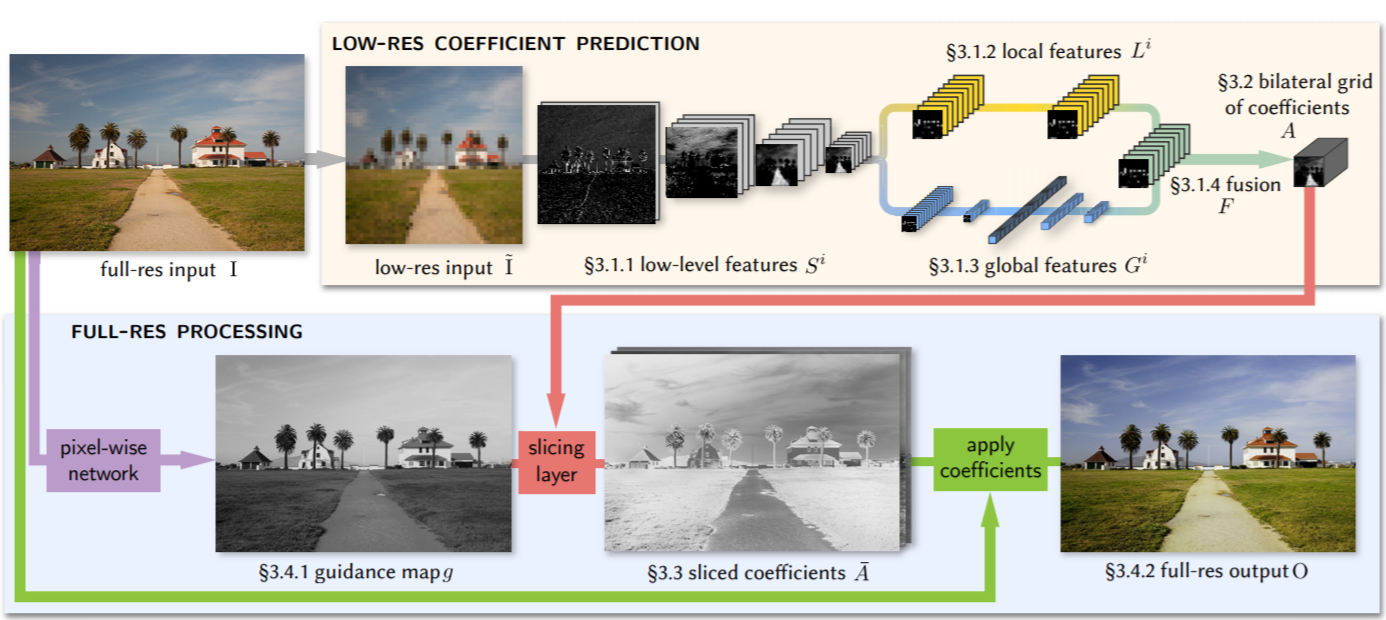
\includegraphics[width=0.9\textwidth]{./images/DeepBilateralLearning01.png}
\caption{}
\end{figure}

\subsection{Low level features:}

\[S^i_{c}[x,y]=\sigma(b^i_{c}+\sum_{x',y',c'}w_{cc'}^i[x',y']S^{i-1}_{c'}[sx+x',sy+y'])\]

\(S^0\)是下采样后得到的分辨率为\(256\times 256\)的低精度图像。

卷积操作,步长为2(\(sx = sy = 2\)),0填充。使用\(n_s\)表示低精度特征卷积层数,\(n_s=4\)。

\subsection{Local features path}

$$
\begin{aligned}
L^0&=S^{n_s} \\
L^i_{c}[x,y]&=\sigma(b^i_{c}+\sum_{x',y',c'}w_{cc'}^i[x',y']L^{i-1}_{c'}[sx+x',sy+y'])
\end{aligned}
$$

卷积操作,步长为1(\(sx = sy = 1\)),0填充。局部特征路径上共两层卷积操作。

\subsection{Global features path}

$$
\begin{aligned}
G^0&=S^{n_s} \\
G^i_{c}[x,y]&=\sigma(b^i_{c}+\sum_{x',y',c'}w_{cc'}^i[x',y']G^{i-1}_{c'}[sx+x',sy+y'])\text{ where } i \in \lbrace 1, 2 \rbrace \\
G^i_{c}&=\sigma(b^i_c+\sum_{x,y,c'}w^i_{cc'}[x,y]G^{i-1}_{c'}[x,y])\text{ where } i \in \lbrace 3, 4, 5 \rbrace
\end{aligned}
$$

先做两次卷积操作,步长为2(\(sx = sy = 2\)),0填充;再做三次全连接操作。

\subsection{Fusion and linear prediction}

$$
\begin{aligned}
F_{c}[x,y]&=\sigma(b_c+\sum_{c'}w'_{cc'}G^{n_G}_{c'}+\sum_{c'}w_{cc'}L_{c'}^{n_L}[x,y]) \\
A_c[x,y]&= b_c+\sum_{c'}F_{c'}[x,y]w_{cc'}
\end{aligned}
$$

\subsection{各层类型与形状信息}

\begin{figure}
\centering
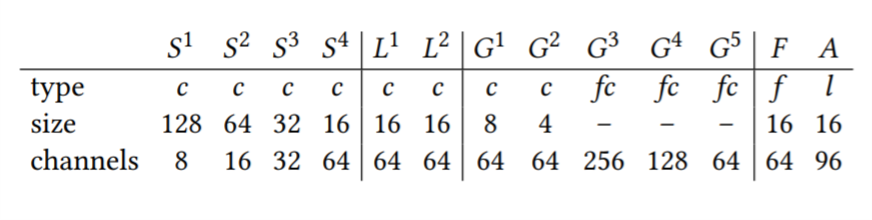
\includegraphics[width=0.9\textwidth]{./images/DeepBilateralLearning02.png}
\caption{}
\end{figure}

\subsection{Guidance map auxiliary network}

$$
\begin{aligned}
\rho_c(x) &= \sum_{i=0}^{15}a_{c,i}\max(x-t_{c,i}, 0)\\
g[x,y] &= b + \sum_{c=0}^{2}\rho_c(\textbf{M}_c^T\cdot \phi_c[x,y]+ b_c')
\end{aligned}
$$

其中\(t_{c,i}\)是阈值,\(a_{c,i}\)是斜率,\(\textbf{M}_{c}^T\)是\(3\times 3\)的颜色变换矩阵,\(b\)和\(b'\)是标量偏置,所有这些参数都可以从另一个网络中学习得到。

\subsection{Upsampling with a trainable slicing layer}

$$
\begin{aligned}
\bar{A}_c[x,y] &= \sum_{i,j,k}\tau(s_x x - i)\tau(s_y y - j)\tau(d\cdot g[x,y]-k)A_{c}[i,j,k]
\end{aligned}
$$

其中\(\tau(\cdot)=\max(1-|\cdot|,0)\),\(s_x=\frac{全分辨率图像宽度}{网格宽度}\),\(s_y=\frac{全分辨率图像高度}{网格高度}\)。

$$
\begin{aligned}
\frac{\partial L}{\partial g[x,y]} &= \frac{\partial L}{\partial \bar{A}_c[x,y]}\frac{\partial \bar{A}_c[x,y]}{\partial g[x,y]} \\
&= \frac{\partial L}{\partial \bar{A}_c[x,y]} \sum_{i,j,k}\tau(s_x x - i)\tau(s_y y - j)\frac{\partial\tau(d\cdot g[x,y]-k)}{\partial g[x,y]}A_{c}[i,j,k]\\
\frac{\partial L}{\partial A_c[i,j,k]}&=\frac{\partial L}{\partial \bar{A}_c[x,y]}\frac{\partial \bar{A}_c[x,y]}{\partial A_c[x,y]}\\
&=\frac{\partial L}{\partial \bar{A}_c[x,y]}\sum_{i,j,k}\tau(s_x x - i)\tau(s_y y - j)\tau(d\cdot g[x,y]-k)
\end{aligned}
$$

\subsection{Assembling the final output}

$$
\begin{aligned}
O_c[x,y]&=\bar{A}_{n_{\phi}+(n_{\phi} + 1)c} + \sum_{c'=0}^{n_{\phi}-1}\bar{A}_{c'+(x_{\phi}+1)c}[x,y]\phi_{c'}[x,y]
\end{aligned}
$$

\subsection{Loss function}

\[L=\frac{1}{|D|}\sum_{i}||f(I_i)-O_i||^2\]

\subsection{Evaluation}

该工作的评估部分采用了7个应用作为基准测试,可以分为三类:

\begin{enumerate}
\def\labelenumi{\arabic{enumi}.}
\item
  近似公开的图像处理管线
\end{enumerate}

\begin{itemize}
\item
  \href{http://graphics.stanford.edu/papers/hdrp/hasinoff-hdrplus-sigasia16-preprint.pdf}{{[}SIGASIA1{]}HDR+},
  a complex hand-engineered photographic pipeline that includes color
  correction, auto-exposure, dehazing(去雾), and tone-mapping. 
\item
  \href{https://people.csail.mit.edu/sparis/publi/2011/siggraph/Paris_11_Local_Laplacian_Filters_lowres.pdf}{{[}SIGGRAPH11{]}The
  Local Laplacian filter}, anedge-preserving,
  multi-scale(yetnon-scale-invariant) operator used for detail
  enhancement(we use two different strengths for the effect).
\item
  \href{https://www.di.ens.fr/willow/pdfscurrent/Aubry14tog.pdf}{{[}TOG14{]}The
  Style Transfer task} (which happens to be based on the Local
  Laplacian).
\item
  \href{http://vis-www.cs.umass.edu/fddb/fddb.pdf}{{[}Technical Report
  10{]}Face brightening task} using a dataset of labeled faces. 
\end{itemize}

\begin{enumerate}
\def\labelenumi{\arabic{enumi}.}
\item
  逆向Photoshop的黑盒动作
\end{enumerate}

\begin{itemize}
\item
  Several different black-box Adobe Photoshop (PS) filters.
\item
  User created PS
  \href{https://designbump.com/photoshop-actions-for-instagram-effects/}{actions}.
\end{itemize}

\begin{enumerate}
\def\labelenumi{\arabic{enumi}.}
\item
  学习摄影师的修图风格
\end{enumerate}

\begin{itemize}
\item
  五位摄影师在\href{http://data.csail.mit.edu/graphics/fivek/}{MIT5K}数据集上修图风格
\end{itemize}

工作效果从近似图像质量(使用PSNR,峰值信噪比进行度量)和执行效率两个方面进行评估。对于前两类应用,选择之前相似的Bilateral
Guided Upsampling(BGU)和 Transfrom
Recipes(TR)作为基准;对于第三类应用,选择之前相似的\href{http://www.sungjuhwang.com/files/hwang12a.pdf}{Hwang@EVCC12}和\href{https://arxiv.org/abs/1412.7725}{Yan@TOG16}作为基准。

\begin{figure}
\centering
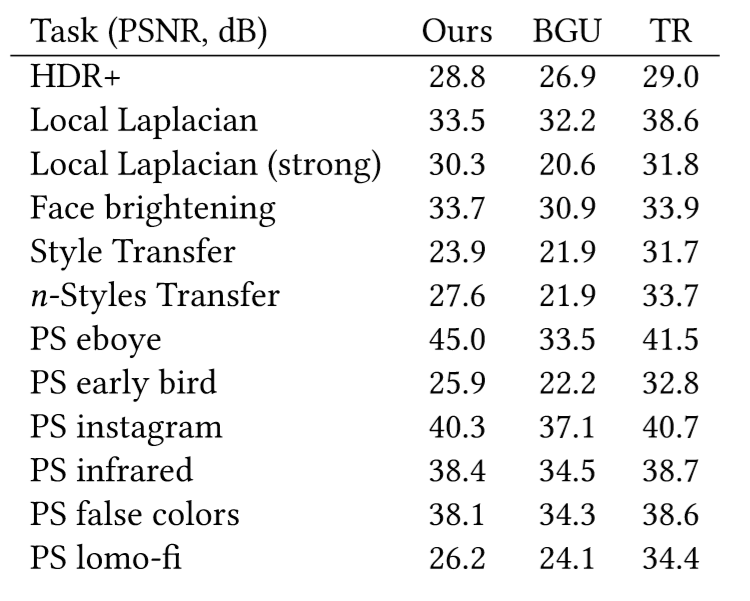
\includegraphics[width=0.9\textwidth]{./images/DeepBilateralLearning03.png}
\caption{}
\end{figure}

执行性能上,实验平台为搭载Android
7.1.1的\href{https://store.google.com/product/pixel_compare}{Google
Pixel phone},处理图像分辨率为1920x1080,刷新频率为40-50Hz。

\begin{enumerate}
\def\labelenumi{\arabic{enumi}.}
\item
  extract 8-bitt preview frames in YUV420 format using the
  \href{https://developer.android.com/reference/android/hardware/camera2/package-summary}{Camera2
  API}
\item
  downsampled to 256x256 and converted into point RGB format, then fed
  into network
\item
  transfer output to the GPU as a set of three 3D RGBA textures, then
  sliced and applied to the full-resolution input to render the final
  processed preview
\end{enumerate}

整体吞吐可以做到20ms一张图,其中14ms在CPU端进行推断,1ms加载系数,18毫秒渲染最终图像(流水线)。比较前两类应用,的确在保证输出图像质量的前提下提高了计算效率,可以达到实时要求。此外计算代价可以做到随着输入规模线性增长。

最后文章比较了之前基于相似想法的两个工作:\href{https://arxiv.org/abs/1505.04597}{{[}MICCAI15{]}U-net}和\href{https://arxiv.org/abs/1511.07122}{{[}CoRR15{]}dialted}。

\begin{figure}
\centering
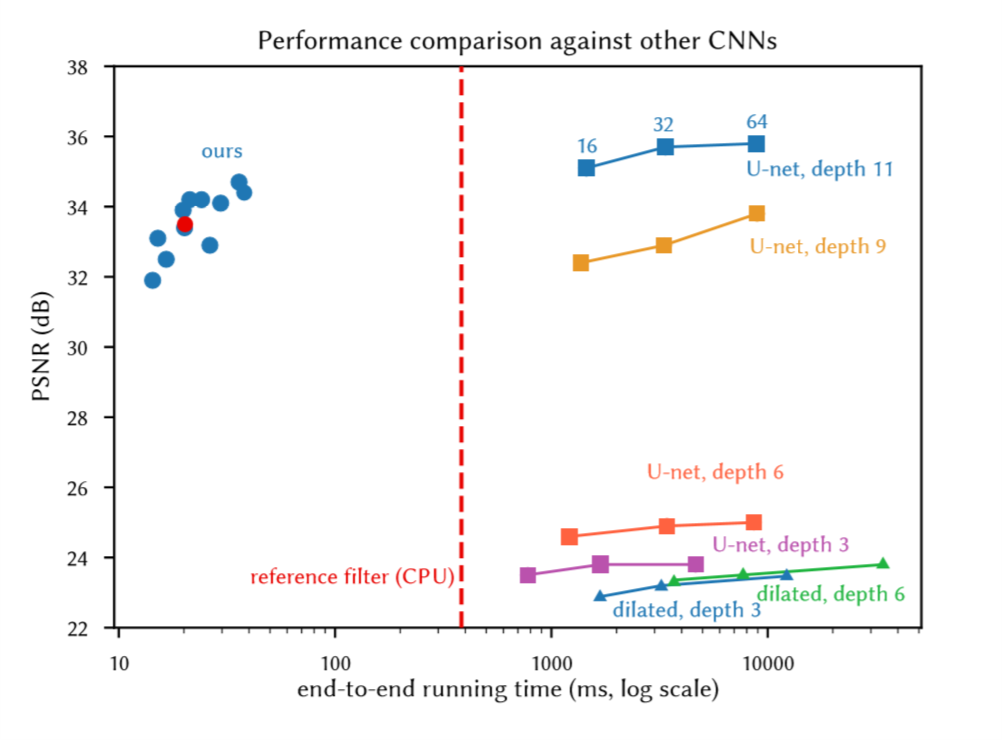
\includegraphics[width=0.9\textwidth]{./images/DeepBilateralLearning04.png}
\caption{}
\end{figure}

注:depth表示网络中向下采样层数量,width表示第一个卷积层中通道数量